%----------------------------------------------------------
\chapter{Архитектура программной реализации}\label{chap3_soft_architecture}
%----------------------------------------------------------

% Вставьте сюда какое-нибудь вступление в главу, я не знаю.
Для описанной в разделе \ref{sec:concept} управляющей структуры была описана логика работы, представленная на рисунке \ref{fig:flowchartExecutionContainer}.
\begin{figure}[!ht]
    \centering
    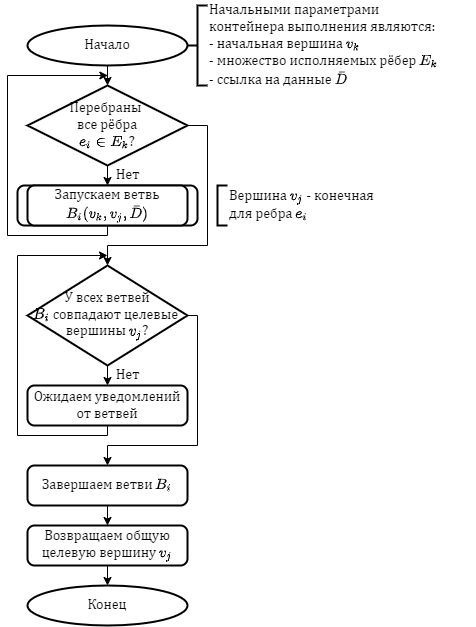
\includegraphics[width=\textwidth]{figures/flowchart.executionContainer.png}
    \caption{Блок-схема алгоритма отслеживания параллельного исполнения ветвей графа}
    \label{fig:flowchartExecutionContainer}
\end{figure}
%----------------------------------------------------------

